\chapter{Diseño e implementación} % Main chapter title

\label{Chapter3} % Change X to a consecutive number; for referencing this chapter elsewhere, use \ref{ChapterX}

\definecolor{mygreen}{rgb}{0,0.6,0}
\definecolor{mygray}{rgb}{0.5,0.5,0.5}
\definecolor{mymauve}{rgb}{0.58,0,0.82}

%%%%%%%%%%%%%%%%%%%%%%%%%%%%%%%%%%%%%%%%%%%%%%%%%%%%%%%%%%%%%%%%%%%%%%%%%%%%%
% parámetros para configurar el formato del código en los entornos lstlisting
%%%%%%%%%%%%%%%%%%%%%%%%%%%%%%%%%%%%%%%%%%%%%%%%%%%%%%%%%%%%%%%%%%%%%%%%%%%%%
\lstset{ %
  backgroundcolor=\color{white},   % choose the background color; you must add \usepackage{color} or \usepackage{xcolor}
  basicstyle=\footnotesize,        % the size of the fonts that are used for the code
  breakatwhitespace=false,         % sets if automatic breaks should only happen at whitespace
  breaklines=true,                 % sets automatic line breaking
  captionpos=b,                    % sets the caption-position to bottom
  commentstyle=\color{mygreen},    % comment style
  deletekeywords={...},            % if you want to delete keywords from the given language
  %escapeinside={\%*}{*)},          % if you want to add LaTeX within your code
  %extendedchars=true,              % lets you use non-ASCII characters; for 8-bits encodings only, does not work with UTF-8
  %frame=single,	                % adds a frame around the code
  keepspaces=true,                 % keeps spaces in text, useful for keeping indentation of code (possibly needs columns=flexible)
  keywordstyle=\color{blue},       % keyword style
  language=[ANSI]C,                % the language of the code
  %otherkeywords={*,...},           % if you want to add more keywords to the set
  numbers=left,                    % where to put the line-numbers; possible values are (none, left, right)
  numbersep=5pt,                   % how far the line-numbers are from the code
  numberstyle=\tiny\color{mygray}, % the style that is used for the line-numbers
  rulecolor=\color{black},         % if not set, the frame-color may be changed on line-breaks within not-black text (e.g. comments (green here))
  showspaces=false,                % show spaces everywhere adding particular underscores; it overrides 'showstringspaces'
  showstringspaces=false,          % underline spaces within strings only
  showtabs=false,                  % show tabs within strings adding particular underscores
  stepnumber=1,                    % the step between two line-numbers. If it's 1, each line will be numbered
  stringstyle=\color{mymauve},     % string literal style
  tabsize=2,	                   % sets default tabsize to 2 spaces
  title=\lstname,                  % show the filename of files included with \lstinputlisting; also try caption instead of title
  morecomment=[s]{/*}{*/}
}



En este capítulo se describe la arquitectura de la aplicación, se muestra cómo interaccionan los distintos procesos entre sí y se explican las estrategias utilizadas para cumplir los requerimientos.

\section{Arquitectura del sistema}
\label{subsec:ArqSistema}
%Explicacion de la arquitectura desarrollada

%El hardware del DASN está basado en un MCU de Texas Instrument, el CC2640R2. Uno de los requisitos del sistema es tener una comunicación inalámbrica BLE 5.0, el protocolo BLE es realmente muy complejo por lo que para implementar esta vía de comunicación se usará el stack BLE que provee texas instrument. El stack BLE de texas instrument está basado en su propio sistema operativo, el TI-RTOS, que es un sistema operativo muy similar al free-RTOS.
%
%Otro de los componentes principales del DASN es el ADC ADS1299, que no es un simple ADC, es todo un front-END, que quiere decir esto, que el propio ADC incorpora internamente un amplificador de ganancia programable para cada canal, un multiplexor de entrada para manejar la configuración de electrodos a utilizar, se puede manejar la inyección de la señal de impedancia, se puede configurar la frecuencia de muestreo y varias cosas más que son muy específicas de este dispositivo. 
%
%Al inicio del proyecto se planteó como uno de los requisitos hacer una capa de HAL para tener un software portable, pero la arquitectura del sistema está fuertemente atada al hardware a utilizar y pensar en cambiar alguno de estos dos componentes significa cambiar todo el proyecto, querer incorporar una capa de HAL para el stack BLE generaría un overhead muy grande y no tiene ningún sentido por lo que pensando en la optimización del código y del tiempo de desarrollo no se implementará dicha capa.
%
%El firmware correrá bajo el sistema operativo de Texas, el TI-RTOS, cada módulo tendrá su tarea asociada del SO y se utilizarán todos los mecanismos de intercomunicación de tareas que ofrece el SO. 
%
%La capa de aplicación estará compuesta por los siguientes componentes de software:
%
%                          DIAGRAMA EN BLOQUES DE LA ARQUITECTURA
%
%Cada uno de estos componentes correrá en una tarea del SO y la comunicación entre los distintos módulos será a través de colas de mensaje transmitiendo los distintos eventos. El sistema será un sistema reactivo donde cada tarea responderá a un evento. Ninguna tarea es bloqueante, es decir, no se quedarán bloqueadas en un punto consumiendo ciclos de CPU. Cuando tengan que esperar algún evento o tiempo se utilizaran herramientas del SO para delegar la CPU a otra tarea que esté en estado Ready. 
%
%
%El hecho de trabajar con el stack Bluetooth embebido en el mismo microcontrolador que maneja todo el dispositivo nos limitó desde un principio en la elección del sistema operativo a utilizar. La API 


% ----------------------------------- INICIO ---------------------------------

La arquitectura esta basada en el sistema operativo TI-RTOS (\textit{Texas Instrument Real Time Opertation System}) propiedad de texas instrument. Esta decisión se tomó ya que el SDK provee una API para comunicarse con el stack Bluetooth basada en este sistema operativo. Si bien creando una capa de abstracción de hardware (HAL) es posible utilizar otros sistemas operativos más generales como el freeRTOS (utilizado en las materias de sistemas operativos en tiempo real I y II), esta tarea no fue contemplada en la planificación ya que no era un requisito para este trabajo. Es una buena práctica no quedar fuertemente ligado a la plataforma de hardware utilizada pero en este caso el tiempo de desarrollo requerido para no utilizar el TI-RTOS no justifica los beneficios.

El stack Bluetooth se encuentra en una biblioteca la cual Texas Instrument no provee su código fuente por temas de política de la compañía. Como se ha dicho previamente provee una API para poder comunicarse con el stack Bluetooth. El stack requiere funcionar en la tarea del sistema operativo de mayor prioridad. Para el correcto funcionamiento del sistema es muy importante que ninguna tarea que hagamos sea bloqueante ya que esto provocaría fallos en la comunicación Bluetooth.

Se planteó una arquitectura modular, donde cada módulo encapsule sus funciones. En la figura \ref{fig:DiagramaEnBloquesArquitectura} podemos ver un diagrama en bloques general donde cada bloque representa un módulo de software.


\vspace{1cm}
\begin{figure}[htbp]
	\centering
	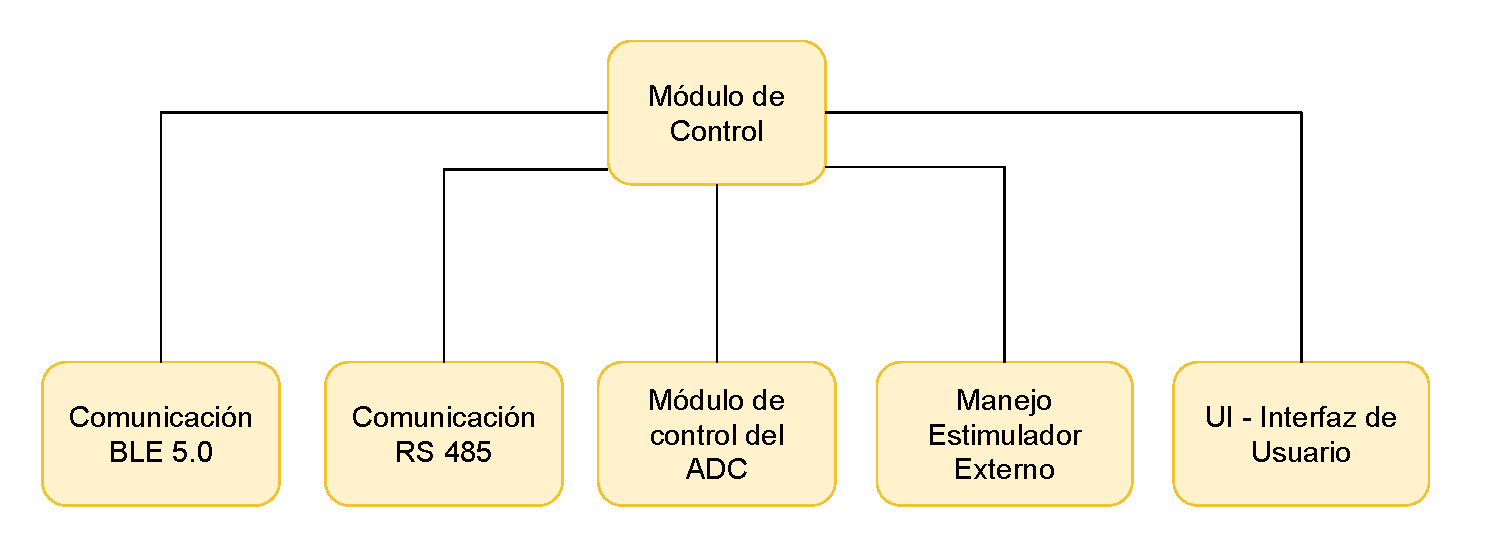
\includegraphics[width=1\textwidth]{./Figures/ArquitecturaSoftware.pdf}
	\caption{Diagrama en bloques de la arquitectura de software.}
	\label{fig:DiagramaEnBloquesArquitectura}
\end{figure}
\vspace{1cm}

%El Módulo de Control es el módulo principal que orquesta todo el sistema

\newpage
\section{Módulo de control}
%Explicación del módulo de control
Este módulo es el módulo principal, esta desarrollado en los archivos DASN\_app.c y DASN\_app.h. Corre en una tarea del sistema operativo y es el encargado de inicializar el hardware y los distintos módulos. Una vez inicializado queda a la espera de recibir eventos a través de la API Event\_pend(), la cual es una función no bloqueante. Se lee el evento recibido y se ejecuta la tarea correspondiente. 

(CONTINUARÁ...)

\section{Módulo BLE}
%Explicación de como funciona el módulo
Como se explicó previamente en la sección \ref{subsec:ArqSistema}, a través de a API vamos a hacer uso del stack Bluetooth. A continuación se detallan las configuraciones principales que se llevaron a cabo para el desarrollo del DASN. 

\subsection{Configuración capa GAP}
Como vimos en la sección \ref{subsec:ConceptosBLE} se le debe asignar un rol al DASN dentro de la capa GAP. El DASN por ser un dispositivo portable necesita anunciarse al resto de los dispositivos y entablar una conexión para transmitir los datos adquiridos. El rol que cumple con estos requisitos es el de un \textit{peripheral}. Para configurar al dispositivo como un \textit{peripheral} en la inicialización del módulo BLE debemos hacer uso de la siguiente API:
\begin{itemize}
\item GAP\_DeviceInit() con el parámetro GAP\_PROFILE\_PERIPHERAL.
\end{itemize}

\subsection{Parámetros de conexión}
En esta sección se describen los parámetros de la conexión. Los parámetros de la conexión son enviados por el dispositivo iniciador de la misma, en nuestro caso el equipo que inicia la conexión siempre es el equipo de registro. Para asegurar un correcto funcionamiento no se puede dejar a elección del equipo de registro los parámetros de conexión. El DASN hace \textit{streaming} de datos, lo que requiere un ajuste exacto de los tiempos. Debe ser el propio DASN quien elija los parámetros de conexión, y esto está contemplado por el stack Bluetooth. Luego de establecerse la conexión el DASN solicita al otro dispositivo cambiar los parámetros de conexión. En el código \ref{codigo:ParametroConn} se muestran los parámetros y la API para actualizar los parámetros en el \textit{stack} Bluetooth.


\begin{lstlisting}[caption= Parámetros de conexión , label=codigo:ParametroConn]	
static void DASN_sendParamUpdate(uint16_t connHandle)
{
    gapUpdateLinkParamReq_t req;

    req.connectionHandle = connHandle;
    req.connLatency = SLAVE_LATENCY;
    req.connTimeout = CONN_TIMEOUT;
    req.intervalMin = MIN_CONN_INTERVAL;
    req.intervalMax = MAX_CONN_INTERVAL;

    // Send parameter update
    bStatus_t status = GAP_UpdateLinkParamReq(&req);
}
\end{lstlisting}

A continuación se describen los parámetros y en la tabla \ref{tab:ParametrosConexion} se muestran los valores asignados a cada uno de ellos:
\begin{itemize}
\item \textit{Connection interval}: es el tiempo entre las conexiones para enviar datos. Este parámetro tiene unidades de 1,25 ms. Acepta valores entre 6 (7,5 ms) y 3200 (4 s).

\item \textit{Peripheral latency}: representa el número máximo de eventos de conexión que un dispositivo se puede saltear. Sirve para minimizar el consumo si no se tiene nueva información a enviar, pero del otro lado de la conexión se tarda más tiempo en detectar un error ya que no se sabe si el paquete se perdió o no fue enviado hasta que se cumpla el tiempo de latencia. Acepta valores entre 0 y 499.

\item \textit{Supervision time-out}: Es el tiempo máximo entre dos eventos de conexión. Si se cumple este tiempo sin que ocurra un evento de conexión, el dispositivo vuelve a un estado desconectado. Este parámetro tiene unidades de 10ms. Acepta valores entre 10 (100 ms) y 3200 (32 s).
\end{itemize}

\begin{table}[h]
\centering
\caption[Parámetros de conexión configurados]{Parámetros de conexión configurados}
\begin{tabular}{l c c}
\toprule
\textbf{Parámetro} & \textbf{Valor} & \textbf{Observaciones}\\
\midrule
MIN\_CONN\_INTERVAL & 6   & Se elije el mínimo valor para\\ 
                    &     & maximizar el ancho de banda\\
                    &     & \\
MAX\_CONN\_INTERVAL & 6   & Se hace igual a MIN\_CONN\_INTERVAL  \\
                    &     & para asegurar  el uso de este valor y que \\
                    &     & no se negocie otro con el \textit{client}\\
                    &     & \\ 
SLAVE\_LATENCY      & 0   & No se permite saltear ninguna conexión. \\
                    &     & \\
CONN\_TIMEOUT       & 200 & En unidades de 10 ms da 2 s. \\

\bottomrule
\hline
\end{tabular}
\label{tab:ParametrosConexion}
\end{table}

\subsection{Configuración capa GATT}
Un dispositivo en la capa GATT puede funcionar como \textit{client} o \textit{server}. Al inicializar el DASN se configura en el stack como \textit{server} ya que dispondrá de las \textit{characteristics} a ser leídas o escritas por el equipo de registro.

Con la API GGS\_SetParameter() y los parámetros correspondientes se configuró el nombre del dispositivo en el servicio GAP GATT. El código \ref{codigo:GAPGATTName} es un extracto del código de inicialización donde vemos como se configura el nombre del dispositivo.

\begin{lstlisting}[caption= Configuración nombre del dispositivo, label=codigo:GAPGATTName]
//Largo del atributo nombre del dispositivo
#define GAP_DEVICE_NAME_LEN		12

//Nombre del dispositivo
static uint8_t attDeviceName[GAP_DEVICE_NAME_LEN] = "DASN V.1.0.0";

//GGS_DEVICE_NAME_ATT indica que vamos a setear el nombre del dispositivo

GGS_SetParameter(GGS_DEVICE_NAME_ATT,GAP_DEVICE_NAME_LEN,attDeviceName);
\end{lstlisting}

\subsection{\textit{Services} Bluetooth configurados}
%Tabla configuración de servicios
El DASN se desarrolló con un único \textit{service}. Se le dió el nombre DATA\_SERVICE el cual se compone de tres \textit{characteristics} 
\begin{itemize}
\item DS\_CMD\_RCV: usada para recibir comandos en el DASN.
\item DS\_CMD\_SND: usada para enviar comandos desde el DASN.
\item DS\_STREAM: usada para enviar el paquete de datos desde el DASN.
\end{itemize}

Cada \textit{service} y \textit{characteristic} requiere un número de identificación (UUID). En el código \ref{codigo:ConfiguracionUUID} se puede ver un extracto del archivo \textit{data\_service.h} que muestra la configuración de los UUID para el \textit{service} del DASN.

\begin{lstlisting}[caption= Configuración UUID , firstnumber=65 , label=codigo:ConfiguracionUUID]	
// Service UUID
#define DATA_SERVICE_SERV_UUID 0x1130

// Cmd rcv Characteristic defines
#define DS_CMD_RCV_ID                 0
#define DS_CMD_RCV_UUID               0x1131
#define DS_CMD_RCV_LEN                1
#define DS_CMD_RCV_LEN_MIN            0

// Cmd snd Characteristic defines
#define DS_CMD_SND_ID                 1
#define DS_CMD_SND_UUID               0x1132
#define DS_CMD_SND_LEN                1
#define DS_CMD_SND_LEN_MIN            0

// Stream Characteristic defines
#define DS_STREAM_ID                  2
#define DS_STREAM_UUID                0x1133
#define DS_STREAM_LEN                 32
#define DS_STREAM_LEN_MIN             0
\end{lstlisting}

\subsection{Tabla de \textit{attributes}}

Los \textit{attributes} se deben declarar en una estructura que Texas llama tabla de \textit{attributes}, en el código \ref{codigo:TablaAtt} podemos ver un extracto del archivo \textit{data\_service.c} en donde vemos la declaración del \textit{service} y de las \textit{characteristics}. Podemos destacar que la \textit{characteristic} DS\_CMD\_RCV tiene permiso de escritura (GATT\_PERMIT\_WRITE) ya que el dispositivo \textit{client} tiene que poder escribir en esta \textit{characteristic} el comando a enviar. En cambio, las \textit{characteristics} DS\_CMD\_SND y DS\_STREAM tienen solo permiso de lectura (GATT\_PERMIT\_READ).

\begin{lstlisting}[caption= Tabla de \textit{attributes} , firstnumber=153 , label=codigo:TablaAtt]
static gattAttribute_t Data_ServiceAttrTbl[] =
{
    // Data_Service Service Declaration
    {
        { ATT_BT_UUID_SIZE, primaryServiceUUID },
        GATT_PERMIT_READ,
        0,
        (uint8_t *)&DataServiceDecl
    },
    // Cmd Rcv Characteristic Declaration
    {
        { ATT_BT_UUID_SIZE, characterUUID },
        GATT_PERMIT_READ,
        0,
        &ds_CmdRcvProps
    },
    // Cmd Rcv Characteristic Value
    {
        { ATT_UUID_SIZE, ds_CmdRcvUUID },
        GATT_PERMIT_WRITE,
        0,
        ds_CmdRcvVal
    },
    // Cmd Snd Characteristic Declaration
    {
        { ATT_BT_UUID_SIZE, characterUUID },
        GATT_PERMIT_READ,
        0,
        &ds_CmdSndProps
    },
    // Cmd Snd Characteristic Value
    {
        { ATT_UUID_SIZE, ds_CmdSndUUID },
        GATT_PERMIT_READ,
        0,
        ds_CmdSndVal
    },
    // CmdSnd CCCD
    {
        { ATT_BT_UUID_SIZE, clientCharCfgUUID },
        GATT_PERMIT_READ | GATT_PERMIT_WRITE,
        0,
        (uint8_t *)&ds_CmdSndConfig
    },
    // Stream Characteristic Declaration
    {
        { ATT_BT_UUID_SIZE, characterUUID },
        GATT_PERMIT_READ,
        0,
        &ds_StreamProps
    },
    // Stream Characteristic Value
    {
        { ATT_UUID_SIZE, ds_StreamUUID },
        GATT_PERMIT_READ | GATT_PERMIT_WRITE,
        0,
        ds_StreamVal
    },
    // Stream CCCD
    {
        { ATT_BT_UUID_SIZE, clientCharCfgUUID },
        GATT_PERMIT_READ | GATT_PERMIT_WRITE,
        0,
        (uint8_t *)&ds_StreamConfig
    },
};

\end{lstlisting}

Otro item a destacar de la tabla de \textit{attributes} es que tanto el DS\_CMD\_SND y DS\_STREAM tienen un \textit{attribute} CCCD (de sus siglas en ingles \textit{Client Characteristic Configuration Descriptor}). Este \textit{attribute} sirve para que la \textit{characteristic} se pueda configurar para que el GATT \textit{server} envíe una notificación al GATT \textit{client} cuando haya cambiado el valor de una \textit{characteristic}. Esta es una configuración muy importante ya que determina la forma de funcionamiento del DASN. El DASN cuando tiene un nuevo dato para enviarle al equipo de registro escribe la \textit{characteristic}, ya sea el dato adquirido o un comando de respuesta, con el valor correspondiente y gracias a esta configuración es que el equipo de registro se entera que hay un nuevo dato. 

\newpage
\section{Módulo de adquisición}
%Explicación del módulo de adquisición
Este módulo es el encargado de manejar la comunicación SPI con el ADS1299. Corre en una tarea independiente y se comunica con el módulo de control a travéz de una cola para pasar los datos adquiridos.


\subsection{Máquina de estados}
%Explicación de la maquina de estados que controla el módulo
%Diagrama máquina de estados

En la figura \ref{fig:DiagramaEstados} se puede ver el diagrama en bloques de la máquina de estados del módulo.

\vspace{1cm}
\begin{figure}[htbp]
	\centering
	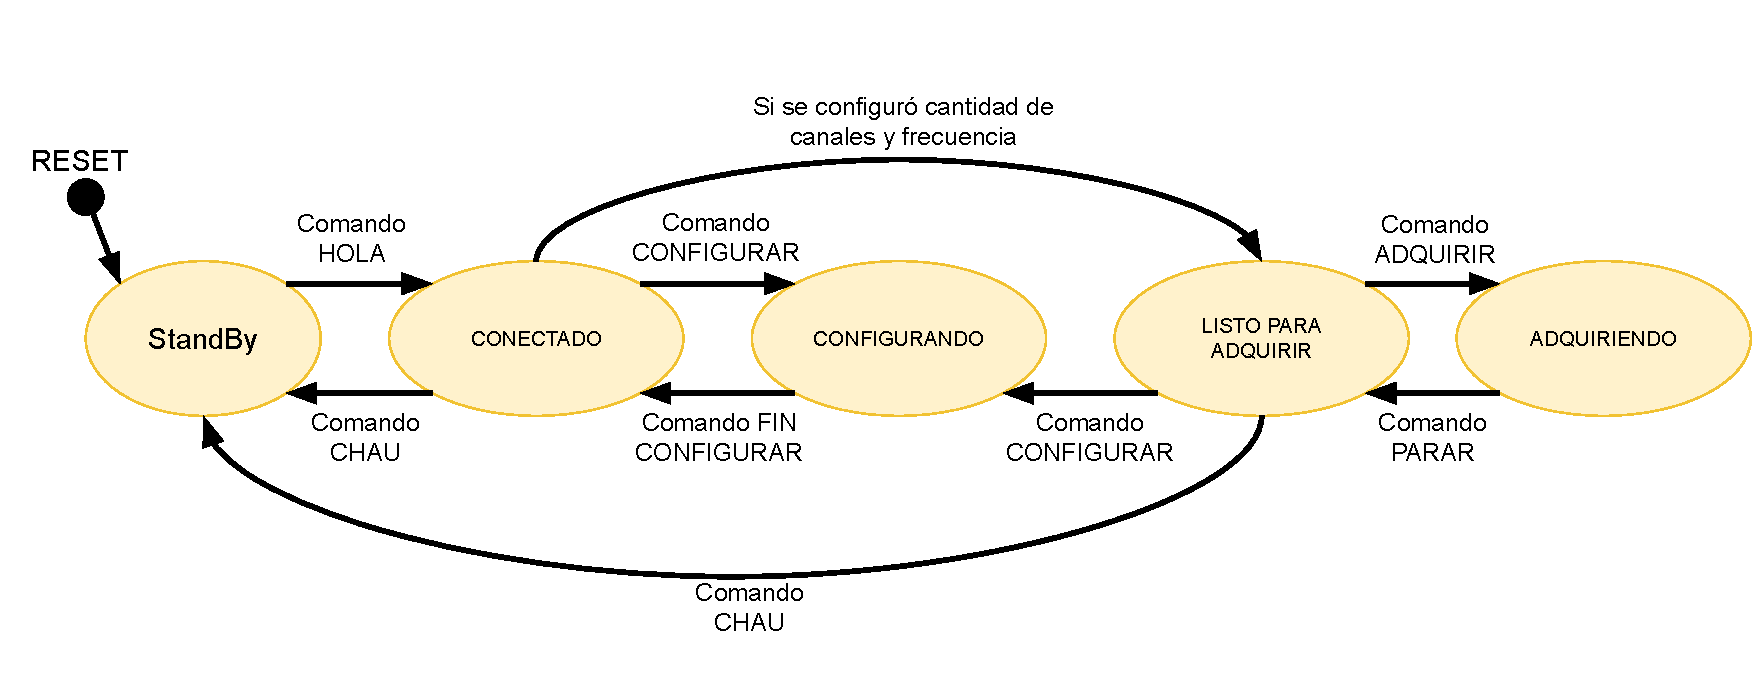
\includegraphics[width=1\textwidth]{./Figures/MEFads1299.pdf}
	\caption{Diagrama en bloques de la máquina de estados del modulo de adquisición.}
	\label{fig:DiagramaEstados}
\end{figure}
\vspace{1cm}

A continuación se describen los estados:
\begin{itemize}
\item STANDBY: estado inicial al reset.
\item CONECTADO: se encienden las fuentes de alimentación y queda a la espera de estar configurado para poder pasar al estado LISTO PARA ADQUIRIR.
\item CONFIGURANDO: se configura frecuencia de muestreo, canales a adquirir y señal de impedancia.
\item LISTO PARA ADQUIRIR: se encuentra configurado y listo para adquirir.
\item ADQUIRIENDO: lee los datos del ADS1299 por SPI y los envía a través de una cola de mensajes al módulo de control.
\end{itemize}

\subsection{Protocolo de comunicación}
%Explicacioón del protocolo de comunicación desarrollado.
%Tabla de comandos
La comunicación entre el \textit{server} y el \textit{client} se realiza leyendo y escribiendo en las \textit{characteristics} DS\_CMD\_SND y DS\_CMD\_RCV. En la tabla \ref{tab:Comandos} se puede ver la lista de comandos con su descripción.
\begin{table}[h]
\centering
\caption[Tabla de comandos]{Tabla de comandos}
\begin{tabular}{l c c}
\toprule
\textbf{Nombre} & \textbf{Valor} & \textbf{Descripción}\\
\midrule
HOLA				&	0x01	&	Inicia la comunicación\\  
OK             	&	0x02	&	Comando ejecutado \\
NO\_OK    		&	0x03	&	No se pudo ejecutar el comando\\
CHAU    			&	0x04	&	Termina la comunicación\\
CONFIG\_INICIAR	&	0x05	&	Inicia configuración\\
CONFIG\_TERMINAR	&	0x06	&	Termina configuración\\
CONFIG\_CH\_ALL\_ON	& 	0x07	&	Habilita todos los canales\\
CONFIG\_CH\_ALL\_OFF &	0x08	&	Deshabilita todos los canales\\
CONFIG\_CH1\_ON    &	0x09	&	Canal 1 habilitado\\
CONFIG\_CH2\_ON    &	0x0A	&	Canal 2 habilitado\\
CONFIG\_CH3\_ON    &	0x0B	&	Canal 3 habilitado\\
CONFIG\_CH4\_ON    &	0x0C	&	Canal 4 habilitado\\
CONFIG\_CH5\_ON    &	0x0D	&	Canal 5 habilitado\\
CONFIG\_CH6\_ON    &	0x0E	&	Canal 6 habilitado\\
CONFIG\_CH7\_ON    &	0x0F	&	Canal 7 habilitado\\
CONFIG\_CH8\_ON    &	0x10	&	Canal 8 habilitado\\
CONFIG\_FREC\_1    &	0x11	&	Configura ADC con frecuencia 1 (16 kHz)\\
CONFIG\_FREC\_2    &	0x12	&	Configura ADC con frecuencia 2 ( 8 kHz)\\
CONFIG\_FREC\_3    &	0x13	&	Configura ADC con frecuencia 3 ( 4 kHz)\\
CONFIG\_FREC\_4    &	0x14	&	Configura ADC con frecuencia 4 ( 2 kHz)\\
CONFIG\_FREC\_5    &	0x15	&	Configura ADC con frecuencia 5 ( 1 kHz)\\
CONFIG\_FREC\_6    &	0x16	&	Configura ADC con frecuencia 6 (500 Hz)\\
CONFIG\_FREC\_7	&	0x17	&	Configura ADC con frecuencia 7 (250 Hz)\\
ADQUIRIR			&	0x18	&	Inicia la adquisición\\
PARAR           	&	0x19	&	Para la adquisición\\
LEER\_ESTADO		&	0x1A	&	Pregunta en que estado se encuentra\\
WAKE\_UP       	&	0x1B	&	Actualiza la máquina de estados\\
ZSIGNAL\_31\_2	&	0x1C	&	Habilita señal de impedancia de 31,2 Hz\\
ZSIGNAL\_7\_8	&	0x1D	&	Habilita señal de impedancia de 7,8 Hz\\
ZSIGNAL\_OFF		&	0x1E	&	Deshabilita señal de impedancia\\
RESET			&	0x1F	&	Reinicia el dispositivo\\

\bottomrule
\hline
\end{tabular}
\label{tab:Comandos}
\end{table}


\subsection{Configuración del puerto SPI}
El puerto SPI se configura en modo \textit{callback}, en este modo la comunicación no es bloqueante. Al momento de inicializar el puerto SPI se carga con un puntero a la función de \textit{callback} que se ejecutará al terminarse una transacción de lectura o escritura del puerto. La tabla \ref{tab:ParamSPI} muestra la configuración del puerto.

\begin{table}[h]
\centering
\caption[Configuración SPI]{Configuración SPI}
\begin{tabular}{l c c}
\toprule
\textbf{Parámetro} & \textbf{Valor} & \textbf{Descripción}\\
\midrule
\textit{bitRate}              & 4000000 & Frecuencia del clock del puerto, ver \ref{subsub:clockSPI}\\ 
\textit{dataSize}             & 8 & Cantidad de bits por palabra\\
\textit{frameFormat}          & SPI\_POL0\_PHA1 & Acorde a hoja de datos del ADS1299 \citep{PART:ADS1299}\\
\textit{mode}                 & SPI\_MASTER & El CC2640R2 maneja el clock\\
\textit{transferMode}         & SPI\_MODE\_CALLBACK & Modo \textit{callback}\\
\textit{transferCallbackFxn}  & transferCallback & Puntero a la función de \textit{callback}\\
\bottomrule
\hline
\end{tabular}
\label{tab:ParamSPI}
\end{table}
\subsubsection{Frecuencia del clock}
\label{subsub:clockSPI}
En figura \ref{fig:DataOut} se muestra la trama de datos de salida del ADS1299. La trama de datos siempre es de 216 bits, no importa si hay canale apagados o no. Esto es así ya que los canales apagados se leen en cero. Considerando que la mayor frecuencia de muestreo es 16 kHz, la frecuencia mínima del clock del SPI debe ser:

\begin{equation}
	\label{eq:bitrate}
	ClockSPI > 216 * 16 kHz = 3,456 MHz
\end{equation}

\vspace{1cm}
\begin{figure}[htbp]
	\centering
	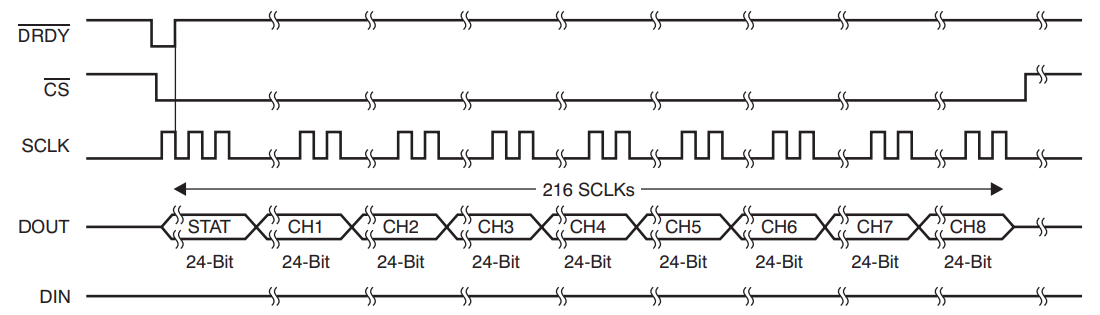
\includegraphics[width=1\textwidth]{./Figures/SPIDataOutput.png}
	\caption{SPI BUS \textit{data output} \protect\footnotemark.}
	\label{fig:DataOut}
\end{figure}
\vspace{1cm}

\footnotetext{Imagen tomada de la hoja de datos del ADS1299 \citep{PART:ADS1299}.}


\subsection{Configuración ADS1299}
%Explicacion de como se configura el dispositivo y los principales registros.
%Tabla de registros
(TBD)

\section{Módulo Interfaz de ususario}
%Explicación del funcionamiento del móodulo
%Pseudocódigo o diagrama en bloques
(TBD)